\documentclass{article}
\usepackage[utf8]{inputenc}
\setlength{\parskip}{5pt} % esp. entre parrafos
\setlength{\parindent}{0pt} % esp. al inicio de un parrafo
\usepackage{listings} % listings
\usepackage{color} %colores
\usepackage{amsmath} % mates
\usepackage[sort&compress,numbers]{natbib} % referencias
\usepackage{url} % que las URLs se vean lindos
\usepackage[top=15mm,left=20mm,right=20mm,bottom=25mm]{geometry} % margenes
\usepackage{hyperref} % ligas de URLs
\usepackage{graphicx} % poner figuras
\usepackage[spanish,es-tabla]{babel} % nombre tablas


\definecolor{mypink}{rgb}{0.976, 0.462, 0.847}
\definecolor{mygray}{rgb}{0.976, 0.980, 0.980}
\definecolor{myblue}{rgb}{0.258, 0.682, 1}
\definecolor{mypink2}{rgb}{0.525, 0.054, 0.4}
\lstset{ 
  backgroundcolor=\color{mygray},
  commentstyle=\color{myblue},
  keywordstyle=\color{mypink}, 
  numberstyle=\tiny\color{mypink}
  stringstyle=\color{mypink2}, 
  breaklines=true,
}

\title{Tarea 6}
\author{Eduardo Navarro}
\date{Octubre 2021}

\begin{document}

\maketitle

\section{Introducción}
En esta tarea, se realizó un análisis sobre los efectos de la vacuna en un sistema multiagente al cual le aplicamos pruebas estadísticas para comprobar nuestro resultado.

\section{Desarrollo}
Con las instrucciones de la tarea \cite{twitchsimu} se hizo un \texttt{for} para las vacunas iniciales y otro \texttt{for} para las repeticiones. Estas modificaciones se hicieron al programa \cite{multiagente}. Así mismo se añadió un \texttt{if} para la inclusión de la probabilidad de recuperados al inicio.

\begin{lstlisting} [language=R, caption= Código para la obtención de vacunados.]
vac<- seq(0.1,0.9,0.1)
g<-(1:30)

datos<-data.frame()

for (pvac in vac) {
  for (rep in g) {
        agentes <- data.frame(x = double(), y = double(),
                          dx = double(), dy = double(),
                          estado  = character())
    for (i in 1:n){
      if (runif(1)<pvac){
        e<-"R"} 
      else if (runif(1) < pi) {
        e <- "I"}
      else{ e <- "S"
      }
\end{lstlisting}

Después se modificó el código para la obtención del máximo de infectados a la vez que su iteración correspondiente. A partir de esto se calculó su porcentaje.

\begin{lstlisting}[language=R, caption= Código para la obtención de los máximos y la iteración correspondiente.]
 maxinf <- 0
    
    for (tiempo in 1:tmax) {
      
      infectados <- dim(agentes[agentes$estado == "I",])[1]
      epidemia <- c(epidemia, infectados)
      
      if (infectados == 0) {
        iteracion=tiempo
        break
      }
      if (max(epidemia)>maxinf){
        maxinf=max(epidemia)
        iteracion=tiempo
      }
      
          porcentaje<-(maxinf/n)*100
    datos <- rbind(datos,c(pvac,maxinf,porcentaje,iteracion))
\end{lstlisting}
Se obtuvieron los datos de la tabla \ref{tabla1} y con ellos se procedió a graficar y a hacer las pruebas estadísticas correspondientes.

\begin{table}[h!]
\centering
\caption{Muestra de datos obtenidos.}
\label{tabla1}
\begin{tabular}{|r|r|r|r|}
\hline
\multicolumn{1}{|l|}{Probabilidad} & \multicolumn{1}{l|}{Máximo} & \multicolumn{1}{l|}{Porcentaje} & \multicolumn{1}{l|}{Tiempo} \\ \hline
0.1 & 30 & 60 & 66 \\ \hline
0.1 & 27 & 54 & 62 \\ \hline
0.1 & 25 & 50 & 44 \\ \hline
0.1 & 28 & 56 & 34 \\ \hline
0.1 & 32 & 64 & 73 \\ \hline
0.1 & 26 & 52 & 80 \\ \hline
0.1 & 29 & 58 & 40 \\ \hline
0.1 & 28 & 56 & 58 \\ \hline
\end{tabular}
\end{table}

\begin{figure} [h!]% figura
\renewcommand{\figurename}{Gráfica}
    \centering
    \caption{ Porcentaje de infectados máximos a partir de los vacunados iniciales.}
    \label{grafica1}
    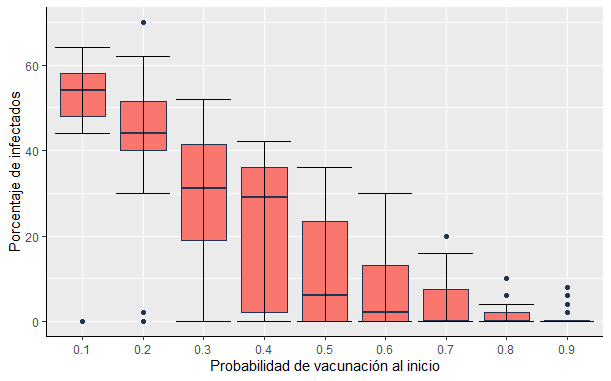
\includegraphics[width=120mm]{grafica1.png} % archivo
\end{figure}

\newpage

\begin{figure} [h!]% figura
\renewcommand{\figurename}{Gráfica}
    \centering
    \caption{Tiempo del máximo de infección obtenido a partir de los vacunados iniciales.}
    \label{grafica2}
    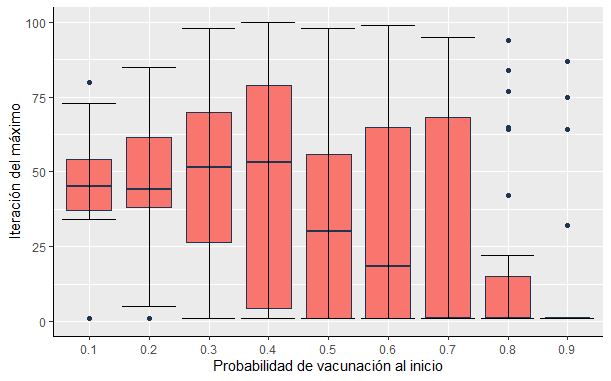
\includegraphics[width=120mm]{grafica2.png} % archivo
\end{figure}

\begin{lstlisting}[language=R, caption= Código para la obtención de las gráficas.]

names(datos)<-c("probabilidad", "maximo", "porcentaje","tiempo")
print(datos)

datos$probabilidad = as.factor(datos$probabilidad)

ggplot(datos, aes(x=probabilidad , y= porcentaje , fill= rep)) + # fill=name allow to automatically dedicate a color for each group
  geom_boxplot(fill = "#F8766D", colour = "#1F3552")+
  stat_boxplot(geom = "errorbar", width = 0.9)+
  theme(axis.line = element_line(colour = "black", size = 0.25))+
  coord_cartesian(ylim = c(0,70))+
  labs(x="Probabilidad de vacunacion al inicio", y= "Porcentaje de infectados")

ggplot(datos, aes(x=probabilidad , y= tiempo , fill= rep)) + # fill=name allow to automatically dedicate a color for each group
  geom_boxplot(fill = "#F8766D", colour = "#1F3552")+
  stat_boxplot(geom = "errorbar", width = 0.9)+
  theme(axis.line = element_line(colour = "black", size = 0.25))+
  coord_cartesian(ylim = c(0,100))+
  labs(x="Probabilidad de vacunacion al inicio", y= "Iteracion del maximo")

\end{lstlisting}

De la gráfica \ref{grafica1} podemos observar una disminución conforme avanzan los vacunados y de la gráfica \ref{grafica2} se aprecia que las iteraciones del máximo se mantienen estables hasta cierto punto. Esto lo comprobamos con las pruebas estadísticas de Shapiro Wilk \cite{shapiro} y Kruskal Wallis\cite{Kruskall} además se realizó la prueba por parejas de Wilcox\cite{pruebass} para observar los resultados de las pruebas anteriores con más detalle.

\newpage

\begin{lstlisting}[language=R, caption= Código de las pruebas estadísticas.]

datos%>%
  group_by(probabilidad) %>%
  summarise(
   
    promedio = mean(porcentaje, na.rm = TRUE),
    desviacion_std = sd(porcentaje, na.rm = TRUE),
    varianza = sd(porcentaje, na.rm = TRUE)^2,
    mediana = median(porcentaje, na.rm = TRUE),
    rango_intercuartil = IQR(porcentaje, na.rm = TRUE)
  )


shapiro.test(datos$porcentaje)
kruskal.test(porcentaje~probabilidad, data=datos)
pairwise.wilcox.test(datos$porcentaje, datos$probabilidad)

datos%>%
  group_by(probabilidad) %>%
  summarise(
   
    promedio = mean(tiempo, na.rm = TRUE),
    desviacion_std = sd(tiempo, na.rm = TRUE),
    varianza = sd(tiempo, na.rm = TRUE)^2,
    mediana = median(tiempo, na.rm = TRUE),
    rango_intercuartil = IQR(tiempo, na.rm = TRUE)
  )

shapiro.test(datos$tiempo)
kruskal.test(tiempo~probabilidad, data=datos)
pairwise.wilcox.test(datos$tiempo, datos$probabilidad)
\end{lstlisting}


\begin{table}[h!]
\centering
\caption{Estadísticas obtenidas para la gráfica \ref{grafica1}.}
\label{tabla2}
\begin{tabular}{|r|r|r|r|r|r|}
\hline
\multicolumn{1}{|l|}{Probabilidad} & \multicolumn{1}{l|}{Promedio} & \multicolumn{1}{l|}{Desviación std} & \multicolumn{1}{l|}{Varianza} & \multicolumn{1}{l|}{Mediana} & \multicolumn{1}{l|}{Rango intercaurtil} \\ \hline
0.1 & 47.4 & 19.6 & 384 & 54 & 10 \\ \hline
0.2 & 41.9 & 16.4 & 268 & 44 & 11.5 \\ \hline
0.3 & 28 & 17.4 & 303 & 31 & 22.5 \\ \hline
0.4 & 22.6 & 16.3 & 265 & 29 & 34 \\ \hline
0.5 & 11.7 & 12.5 & 157 & 6 & 23.5 \\ \hline
0.6 & 7.07 & 8.78 & 77.2 & 2 & 13 \\ \hline
0.7 & 4.6 & 6.26 & 39.2 & 0 & 7.5 \\ \hline
0.8 & 1.27 & 2.26 & 5.1 & 0 & 2 \\ \hline
0.9 & 0.667 & 1.92 & 3.68 & 0 & 0 \\ \hline
\end{tabular}
\end{table}

\newpage

\begin{table}[h!]
\centering
\caption{Resultados de la prueba Shapiro–Wilk para la gráfica \ref{grafica1}.}
\label{tabla3}
 \begin{tabular}{|c|c|c|}
    \hline
    W & P  \\
    \hline
    0.81153 & $2.2\times 10^{-16}$ \\
    \hline
\end{tabular}
\end{table}

\begin{table}[h!]
\centering
\caption{Resultados de la prueba Kruskal-Wallis para la gráfica \ref{grafica1}.}
\label{tabla4}
 \begin{tabular}{|c|c|c|}
    \hline
   H(8) & p-value \\
    \hline
    145.93 & $2.2\times 10^{-16}$ \\
    \hline
\end{tabular}
\end{table}

\begin{table}[h!]
\centering
\caption{Resultados de la prueba por parejas de Wilcox para la gráfica \ref{grafica1}.}
\label{tabla5}
\begin{tabular}{|l|r|r|r|r|r|r|r|r|}
\hline
 & \multicolumn{1}{l|}{0.1} & \multicolumn{1}{l|}{0.2} & \multicolumn{1}{l|}{0.3} & \multicolumn{1}{l|}{0.4} & \multicolumn{1}{l|}{0.5} & \multicolumn{1}{l|}{0.6} & \multicolumn{1}{l|}{0.7} & \multicolumn{1}{l|}{0.8} \\ \hline
0.2 & 0.04581 &  &  &  &  &  &  &  \\ \hline
0.3 & $6.7\times 10^{-5}$ & 0.00828 &  &  &  &  &  &  \\ \hline
0.4 & $9.4\times 10^{-6}$ & $5.5\times 10^{-5}$ & 0.55180 &  &  &  &  &  \\ \hline
0.5 & $3.4\times 10^{-6}$ & $3.1\times 10^{-7}$ & 0.00240 & 0.03243 &  &  &  &  \\ \hline
0.6 & $4.5\times 10^{-6}$ & $1.7\times 10^{-7}$ & 0.00028 & 0.00664 & 0.55180 &  &  &  \\ \hline
0.7 & $1.4\times 10^{-6}$ & $6.8\times 10^{-8}$ & $3.1\times 10^{-5}$ & 0.00082 & 0.26471 & 0.55180 &  &  \\ \hline
0.8 & $6.2\times 10^{-7}$ & $1.4\times 10^{-8}$ & $3.5\times 10^{-6}$ & $6.4\times 10^{-5}$ & 0.03243 & 0.03243 & 0.37241 &  \\ \hline
0.9 & $5.5\times 10^{-8}$ & $1.5\times 10^{-9}$ & $1.4\times 10^{-7}$ & $1.9\times 10^{-6}$ & 0.00083 & 0.00049 & 0.03135 & 0.31388 \\ \hline
\end{tabular}
\end{table}

\begin{table}[h!]
\centering
\caption{Estadísticas obtenidas para la gráfica \ref{grafica2}}
\label{tabla6}
\begin{tabular}{|r|r|r|r|r|r|}
\hline
\multicolumn{1}{|l|}{Probabilidad} & \multicolumn{1}{l|}{Promedio} & \multicolumn{1}{l|}{Desviación std} & \multicolumn{1}{l|}{Varianza} & \multicolumn{1}{l|}{Mediana} & \multicolumn{1}{l|}{Rango intercaurtil} \\ \hline
0.1 & 43.4 & 20.2 & 409 & 45 & 17 \\ \hline
0.2 & 46.9 & 19.3 & 374 & 44 & 23.2 \\ \hline
0.3 & 49.4 & 32.1 & 1031 & 51.5 & 43.2 \\ \hline
0.4 & 48.9 & 35.8 & 1284 & 53 & 74.8 \\ \hline
0.5 & 34.6 & 35.6 & 1264 & 30 & 54.8 \\ \hline
0.6 & 33.5 & 35.3 & 1248 & 18.5 & 64 \\ \hline
0.7 & 30.2 & 37 & 1370 & 1 & 67.2 \\ \hline
0.8 & 16.9 & 29 & 840 & 1 & 14 \\ \hline
0.9 & 9.47 & 23.2 & 540 & 1 & 0 \\ \hline
\end{tabular}
\end{table}

\begin{table}[h!]
\centering
\caption{Resultados de la prueba Shapiro–Wilk para la gráfica \ref{grafica2}}
\label{tabla7}
 \begin{tabular}{|c|c|c|}
    \hline
    W & P  \\
    \hline
    0.85484 & $3.1\times 10^{-15}$ \\
    \hline
\end{tabular}
\end{table}


\begin{table}[h!]
\centering
\caption{Resultados de la prueba Kruskal-Wallis para la gráfica \ref{grafica2}.}
\label{tabla8}
 \begin{tabular}{|c|c|c|}
    \hline
   H(8) & p-value \\
    \hline
    51.479 & $2.1\times 10^{-8}$ \\
    \hline
\end{tabular}
\end{table}

\newpage

\begin{table}[h!]
\centering
\caption{Resultados de la prueba por parejas de Wilcox para la gráfica \ref{grafica2}}
\label{tabla9}
\begin{tabular}{|c|r|r|r|r|r|r|r|r|}
\hline
 & \multicolumn{1}{c|}{0.1} & \multicolumn{1}{c|}{0.2} & \multicolumn{1}{c|}{0.3} & \multicolumn{1}{c|}{0.4} & \multicolumn{1}{c|}{0.5} & \multicolumn{1}{c|}{0.6} & \multicolumn{1}{c|}{0.7} & \multicolumn{1}{c|}{0.8} \\ \hline
0.2 & 1 &  &  &  &  &  &  &  \\ \hline
0.3 & 1 & 1 &  &  &  &  &  &  \\ \hline
0.4 & 1 & 1 & 1 &  &  &  &  &  \\ \hline
0.5 & 1 & 1 & 1 & 1 &  &  &  &  \\ \hline
0.6 & 1 & 1 & 1 & 1 & 1 &  &  &  \\ \hline
0.7 & 1 & 1 & 0.66906 & 0.83667 & 1 & 1 &  &  \\ \hline
0.8 & 0.00897 & 0.00069 & 0.00343 & 0.01128 & 1 & 0.78906 & 1 &  \\ \hline
0.9 & $3.8\times 10^{-5}$ & $2\times 10^{-6}$ & $1.2\times 10^{-5}$ & $5.7\times 10^{-5}$ & 0.01254 & 0.00713 & 0.15303 & 1 \\ \hline
\end{tabular}
\end{table}

\section{Conclusiones}
De esta actividad se concluye que las vacunas son muy importantes en el control epidemiológico por ello la importancia de la aplicación en este tipo de situaciones es muy relevante. En la gráfica \ref{grafica1} se pudo apreciar como los infectados disminuían de forma drástica con cada aumento en la probabilidad de aplicación. Y en la grafica \ref{grafica2} se pudo apreciar el tiempo máximo que hay antes de llegar al pico de infección el cual disminuía conforme se avanzaba en la vacunación debido a que cada vez quedaban menos suceptibles y la epidemia terminaba más rápido. Con las pruebas estadísticas confirmamos que para la gráfica \ref{grafica1} los datos no tienen una distribución normal y las medidas de sus medias no son todas iguales. Del mismo modo ocurre algo similar para la gráfica \ref{grafica2} en donde gracias a la prueba de Wilcox podemos ver que a partir de la probabilidad de 0.6 dejan de considerarse iguales lo que nos indica un decaimiento rápido de la epidemia a partir de ese punto.

\bibliography{referencias}
\bibliographystyle{plainnat}
\end{document}
